\section{Implementation}
\subsection{The Physical Setup (The Brewery Machine)}

The machine can produce different kinds of beer depending on the recipe
used. The beer is produced in batches which have their own batch id. When 
producing a batch the recipe, quantity, speed and batch id can be configured by 
an external system. When a batch has been produced the quality inspection system 
measures the quality for future use. These values are accessible in the machines 
SCADA system. The SCADA system monitors and supervises both the machines PLC 
system and the internal sensors PLC system as well as the quality inspection 
system.

\myparagraph{Sensors}
To ensure the most optimal environment beer production the 
machine is equipped with three sensors that measure the environment while 
production is happening. This data is useful as it gives insight into the 
internal environment of the machine while producing products. Currently, it 
measures temperature, humidity and vibration. The machine itself is not able to 
collect these data and are collected by an external system.

\myparagraph{Quality Inspection System}
To make it possible to calculate an error function, the system is 
equipped with a sophisticated quality inspection system, QIS. This system is key to 
optimising the production by giving data about the different error functions of 
the configurations so that they can be configured otherwise to maximise 
production. Each produced product is inspected and if the quality is low enough
the product will fail. When a batch is finished the QIS will output the amount 
of failed and passed products. The result is then used to calculate the error
function.


\subsection{The Simulator}
The group is going to use the simulator software to test the software during the
development cycle.
It is important to note that the simulator is not a replacement of the machine
since there is only so much randomness and correctness you can get from a 
simulator. 
It is still very important to have the simulator, when making prototypes and 
performing multiple tests on it, so any regressions won't be pushed to 
the production system(the beer machine).


\subsection{Dashboard}
The user interacts with the dashboard, seen in Figure \ref{figure:dashboard}and
through it the user can see what the machine is producing and information about
the production. The user can also interact with the dashboard, as they can start
and stop the machine and press buttons to see live data represented in graphs.
The user is able to query batches for the machine to produces, as well as see
the batch history, to quickly get an overview over produced batches and its data.\\

\begin{figure}[ht]
	\centering
	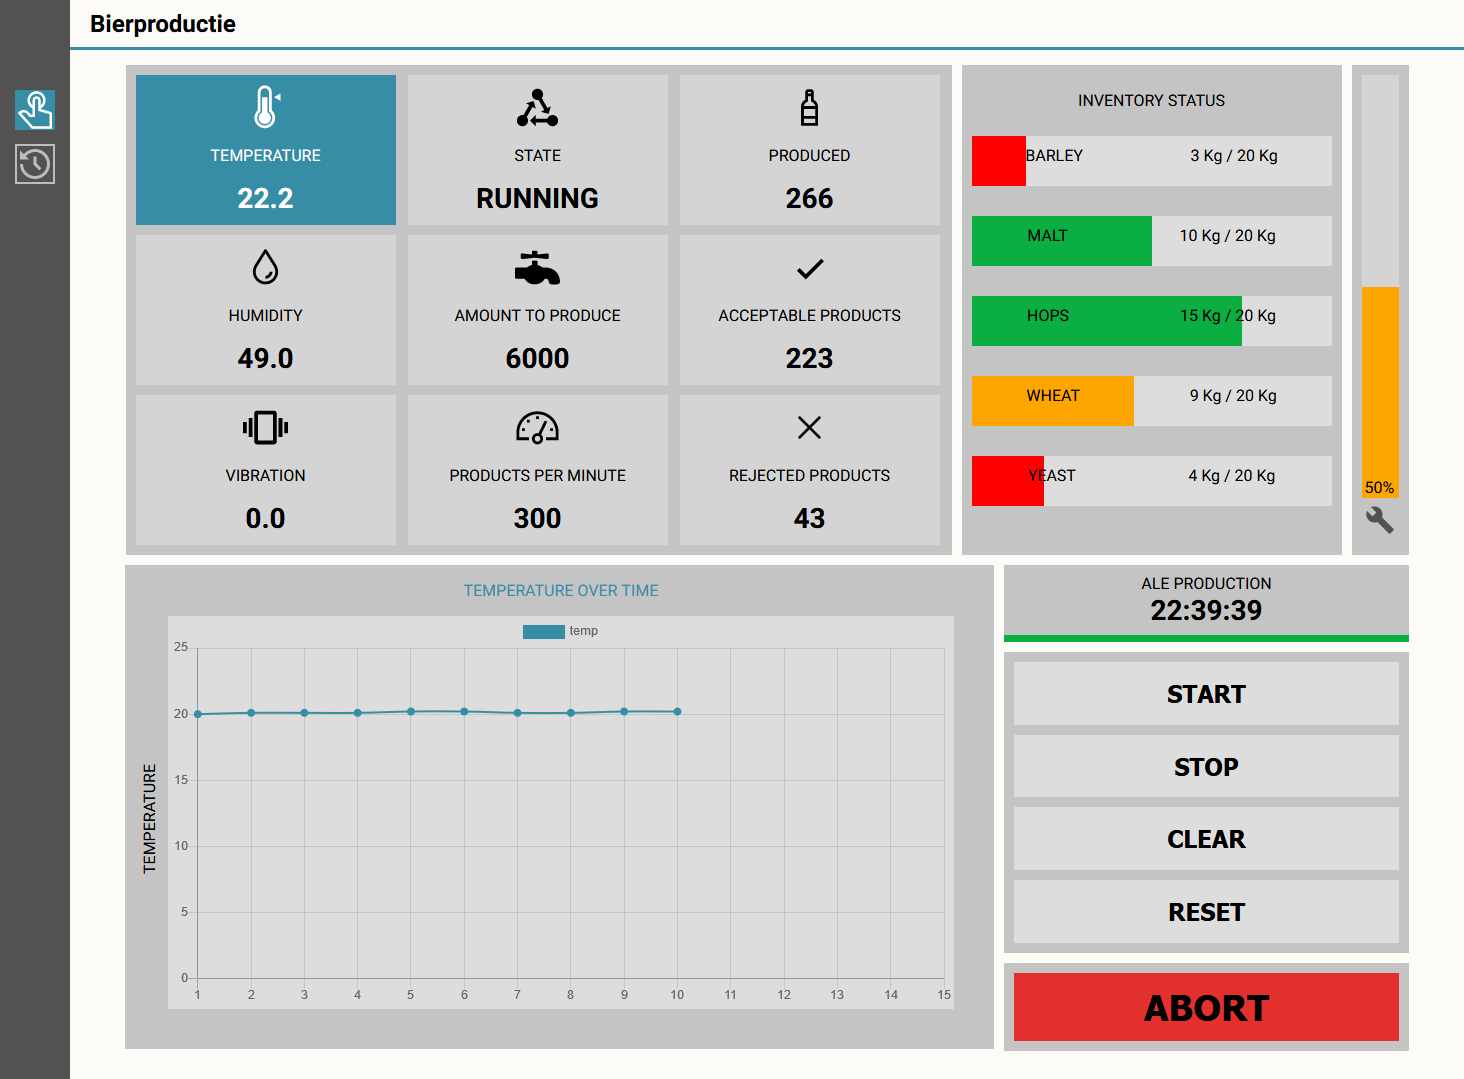
\includegraphics[width=1\linewidth]{images/dashboard.png}
	\caption{Dashboard}
	\label{figure:dashboard}
\end{figure}

The dashboard is implemented using web based technology, so it can run on many
machines without installing any software, apart from a modern browser that is
running JavaScript. It is implemented using HTML, CSS and JavaScript, and it
uses two separate libraries for making graphs and getting icons for the buttons.

\subsection{REST API}

\subsection{Database}

\subsection{OPC-UA-Client}
The OPC-UA-client handles the data from the machine and sends it to the API. It 
is written in Java and uses the Milo library to create a client that connects to 
the machines OPC-UA-server. The OPC-UA-client is able to subscribe to 
information on the server and send it to the API that stores it in the database.
The client also controls the machine while it collects data, as it creates and
runs batches it gets from the dashboard through the API. The client sends live
data to the dashboard via the API using subscriptions. These subscriptions sends
data to the API every time a change appears and the API then forwards it to the
dashboard. The client creates 6 subscriptions when started, they monitor
temperature, vibration, humidity, machine-state,  current defective products and
current processed products. \\

The data is also stored in an object called Batch in the client. The Batch class
has properties corresponding to the values the API uses as well as logic to
process the data. This logic includes OEE calculation and JSON exportation. In
the start of a batch, when the user has configured the desired production, the
data is sent to the client to create a Batch object. The Batch object is then
run with the BatchHandler class, and while the batch is being produced, the
subscriptions will add data to the object. When done the Batch object will run
through its logic and finally export itself as a JSON so it can be sent to the
API. 


\subsection{Overall Equipment Effectiveness}
When a batch is complete, the calculation of the OEE takes place, and the data
stored in the batch class is used for this.\\

For this project, the planned production time can not be estimated properly, as
too many variables are unknown (shift lengths,the time it takes to refill
ingredients, the time it takes to do maintenance work etc.). Therefore, it has
been chosen to use the time it takes to produce a batch. The calculation can be
seen below.

\[PlannedProductionTime = \left(\frac{AmountToProduce}{MachineSpeed}\right)\cdot60\]\\

Where the amount to produce divided by the machine speed gives us the production
time in minutes, as the machine speed is products per minute. This can be
multiplied by 60 to give the production time in seconds. The production time
divided by the amount to produce then gives the ideal cycle time.

\[IdealCycleTime = \frac{PlannedProductionTime}{AmountToProduce}\]\\

When these two have been calculated, it is possible to calculate the OEE using
Equation \ref{eq:OEE}.

\[OEE = \left(\frac{AcceptedProducts\cdot{IdealCycleTime}}{PlannedProductionTime}\right)\cdot100\]\\

This gives the overall equipment effectiveness in percentage, which is used to
evaluate if the production can be optimised further. It should be noted that
the result from this calculation is only indicative, as neither quality,
performance or availability can be assessed from this.

To give an example on how a calculation with real values would look like, take
the values: amount to produce = 100, machine speed = 200, accepted products = 97.

\[PlannedProductionTime = \left(\frac{100}{200}\right)\cdot60 = 30\]

\[IdealCycleTime = \frac{30}{100}=0,30\]

\[OEE = \left(\frac{97\cdot0,30}{30}\right)\cdot100 = 97\%\]\\

The OEE for this specific batch would be 97\%, which means that the production
line is optimised to the point where it would be hard to optimise it further.

\subsection{Error Function}
The error function associated with each product type is to be estimated. For
this several batches should be produced to have some data to calculate on. The
values used to estimate the error function is the amount of products to produce,
the machine speed and the amount of rejected products. These values are used to
make a function expression, that resembles the error function. 


\subsection{Optimal Production Speed}
Pilsner:\\
\[y = -0,0003x3 + 0,0291x2 - 0,95x + 107,38\]
\[R^2 = 0,9916\]

Wheat:\\
\[y = -5E-05x3 + 0,0077x2 - 1,3163x + 103,63\]
\[R^2=0,9983\]

IPA:\\
\[y = 0,0001x3 - 0,0548x2 + 3,7529x + 28\]
\[R^2=0,9981\]

Stout:\\
\[y = 0,0002x3 - 0,0319x2 + 1,551x + 32,929\]
\[R^2=0,9331\]

Ale:\\
\[y = 2E-05x3 - 0,0099x2 + 0,5615x + 90,814\]
\[R^2== 1\]

Alcohol free:\\
\[fy = -3E-05x3 + 0,0021x2 - 0,4464x + 90\]
\[R^2=0,9935\]


this can be used to find the optimal production speed for each product type. 